\documentclass[letterpaper,10pt]{article}
\usepackage{graphicx}
\usepackage{listings}
\usepackage{fullpage}
\usepackage{fixltx2e}
\usepackage{multirow}
\usepackage{amssymb,amsmath}
\usepackage{mathtools}
\usepackage[hyperfootnotes=false,hidelinks]{hyperref}
\usepackage{url}
\usepackage{subfig}
\usepackage{relsize}
\usepackage{enumitem}
\usepackage{booktabs}
\usepackage{sectsty}
%\usepackage{natbib}
%\sectionfont{\fontsize{14}{16}\selectfont}
%\usepackage{empheq}
\usepackage[x11names]{xcolor}
%\numberwithin{figure}{section}
%\numberwithin{table}{section}
\numberwithin{equation}{section}
\usepackage{fancyhdr}
\setlength{\headheight}{14pt}
\pagestyle{fancy}
\headsep = 20pt
\linespread{1.0}
\setlength{\parskip}{0.85\baselineskip}
\setlength{\parindent}{0pt}

\renewcommand{\arraystretch}{1.2}
\usepackage{xcolor}
\lstset{basicstyle=\ttfamily,
  showstringspaces=false,
  commentstyle=\color{red},
  keywordstyle=\color{blue}
}

% Custom hyphenation
\hyphenation{tur-bu-lence}
\hyphenation{Rey-nolds}

\def \d {\mathrm{d}}
\newcommand{\dd}[2]{\frac{\d #1}{\d #2}}
\newcommand{\pp}[2]{\frac{\partial #1}{\partial #2}}
\newcommand{\dprime}[1]{^{\prime\prime #1}}
\newcommand{\ol}[1]{\overline{#1}}
\newcommand{\oll}[1]{\overline{#1}_\lambda}
\newcommand{\wt}[1]{\widetilde{#1}}
\newcommand{\wtl}[1]{\widetilde{#1}_\lambda}
\newcommand{\wh}[1]{\widehat{#1}}

% For multiletter symbols
\newcommand\Real{\mbox{Re}} % cf plain TeX's \Re and Reynolds number
\newcommand\Imag{\mbox{Im}} % cf plain TeX's \Im
\newcommand\Rey{\mbox{\textit{Re}}}  % Reynolds number
\newcommand\Pran{\mbox{\textit{Pr}}} % Prandtl number, cf TeX's \Pr product
\newcommand\Pen{\mbox{\textit{Pe}}}  % Peclet number
\newcommand\Da{\mbox{\textit{Da}}}   % Damkohler number
\newcommand\Ka{\mbox{\textit{Ka}}}   % Karlovitz number
\newcommand\Ai{\mbox{Ai}}            % Airy function
\newcommand\Bi{\mbox{Bi}}            % Airy function

\begin{document}

\fancyhf{}
\fancyhead[L]{\textit{PyFlow} Numerics}
\fancyhead[R]{J.F.\ MacArt and J.A.\ Sirignano (\today)}
\fancyfoot[C]{\thepage}


% -----------------------------------------------------------------
\section{Forward Equations}

For an incompressible fluid, the equations governing the conservation
of mass and momentum are
\begin{align}
  \pp{u_j}{x_j} &= 0, \label{eq.mass}\\
  \pp{u_i}{t} &= -\pp{u_iu_j}{x_j} -\frac{1}{\rho}\pp{p}{x_i} + B_i, \label{eq.mom}
\end{align}
respectively, where $\rho$ is the constant fluid density, $u_i$ is the
$i$\textsuperscript{th} velocity component, and $p$ is the
hydrodynamic pressure. Summation over repeated indices is implied. The
viscous flux is
\begin{equation}
  B_i \equiv
  \frac{\mu}{\rho}\pp{}{x_j}\left(\pp{u_i}{x_j}+\pp{u_j}{x_i} -
  \frac{1}{3}\pp{u_k}{x_k}\delta_{ij}\right),
\end{equation}
in which $\mu$ is the constant viscosity and $\delta_{ij}$ is the
Kronecker delta. Note that the assumption of constant $\rho$ and $\mu$
is not strictly necessary for an incompressible fluid.


\subsection{Temporal Discretization}

The governing equations are solved using Chorin's fractional-step
scheme. The system is discretized in time using the explicit Euler
method. In the fractional-step scheme, a ``predicted'' velocity field
$u_i^*$ is computed according to Eq.~\eqref{eq.mom} without the
pressure derivative, \textit{i.e.},
\begin{equation}
  u_i^* = u_i^t - \Delta t\left(\pp{u_iu_j}{x_j} - B_i\right) + \mathcal{O}(\Delta t).
  \label{eq.predictor}
\end{equation}
A Poisson equation is solved to obtain a pressure field that enforces
the divergence-free condition on the velocity field
[Eq.~\eqref{eq.mass}],
\begin{equation}
  \frac{\partial^2 p^*}{\partial x_j^2} = \frac{\rho}{\Delta t}\pp{u_j^*}{x_j}.
  \label{eq.poisson}
\end{equation}
Finally, a ``corrected'' velocity field is obtained by applying the
pressure correction:
\begin{equation}
  u_i^{t+1} = u_i^* - \frac{\Delta t}{\rho}\pp{p^*}{x_i} + \mathcal{O}(\Delta t).
  \label{eq.corrector}
\end{equation}


\subsection{Spatial Discretization}

The system is discretized in space using a fully-staggered grid, in
which the velocity components are located at cell faces and the
pressure is located at cell centers. A uniform mesh is assumed.

Convective terms are discretized in ``divergence form,'' as they
appear in Eq.~\eqref{eq.mom}, due to several desirable conservation
properties on the staggered grid (Morinishi \textit{et al.},
\textit{JCP} 143, 1998). Let us denote the $x,y,z$ components of
velocity as $u_1,u_2,u_3=u,v,w$, respectively. No longer implying
summation over repeated indices, we can write the discretized
convective terms for the $u_1=u$ velocity component at a point
$(i,j,k)$ as
\begin{align}
  \begin{split}
  \left(\pp{uu}{x} + \pp{uv}{y} + \pp{uw}{z}\right)_{i,j,k} &=
  \left(\mathrm{Conv}_{11} + \mathrm{Conv}_{12} + \mathrm{Conv}_{13}\right)_{i,j,k} \\
  &= (\mathrm{grad\_x})\left[u_{i,j,k}^{I,xm}u_{i,j,k}^{I,xm} - u_{i-1,j,k}^{I,xm}u_{i-1,j,k}^{I,xm}\right] \\
  &+ (\mathrm{grad\_y})\left[u_{i,j+1,k}^{I,y}v_{i,j+1,k}^{I,x} - u_{i,j,k}^{I,y}v_{i,j,k}^{I,x}\right] \\
  &+ (\mathrm{grad\_z})\left[u_{i,j,k+1}^{I,z}w_{i,j,k+1}^{I,x} - u_{i,j,k}^Iw_{i,j,k}^{I,x}\right],
  \label{eq.forward_conv}
  \end{split}
\end{align}
where interpolated velocities are defined as
\begin{align*}
  u_{i,j,k}^{I,xm} &= \frac{1}{2}\left(u_{i+1,j,k} + u_{i,j,k}\right), \\
  u_{i,j,k}^{I,y} &= \frac{1}{2}\left(u_{i,j,k} + u_{i,j-1,k}\right), \\
  u_{i,j,k}^{I,z} &= \frac{1}{2}\left(u_{i,j,k} + u_{i,j,k-1}\right), \\
  v_{i,j,k}^{I,x} &= \frac{1}{2}\left(v_{i,j,k} + v_{i-1,j,k}\right), \\
  w_{i,j,k}^{I,x} &= \frac{1}{2}\left(w_{i,j,k} + w_{i-1,j,k}\right),
\end{align*}
and $(\mathrm{grad\_x})$, etc., contain the denominators of the
derivative operators. The order of interpolation and differentiation
in the discretized convective terms will be important in the
derivation of the discrete-exact adjoint equations.




% -----------------------------------------------------------------
\section{Adjoint Equations}

A loss function $\mathcal{L} = g(u^T,v^T,w^T)$ may be defined, where
the superscript $(\cdot)^T$ denotes the solution at a final time
$T$. A typical loss function is the mean-squared error (MSE). The
adjoint of the velocity field at an intermediate time $t$ is then
defined as the gradient of the loss function with respect to the
forward solution at time $t$:
\begin{equation}
  \wh{u}^t \equiv \pp{\mathcal{L}}{u^t},\quad \wh{v}^t \equiv
  \pp{\mathcal{L}}{v^t},\quad \wh{w}^t \equiv \pp{\mathcal{L}}{w^t}.
  \label{eq.adj}
\end{equation}


\subsection{Temporal Discretization}
The adjoint field is advanced in reverse time over the range
$t\in[T-1,0]$. Using dummy indices $(m,n,p)\in (N_x,N_y,N_z)$, the
adjoint of the $u$-component of velocity at a point
$(i,j,k)\in (N_x,N_y,N_z)$ is written using the chain rule on $\mathcal{L}$ and
substituting Eq.~\eqref{eq.adj}:
\begin{equation}
  \wh{u}_{i,j,k}^t = \sum_{m,n,p}\left(
  \wh{u}_{m,n,p}^{t+1}\pp{u_{m,n,p}^{t+1}}{u_{i,j,k}^t} +
  \wh{v}_{m,n,p}^{t+1}\pp{v_{m,n,p}^{t+1}}{u_{i,j,k}^t} +
  \wh{w}_{m,n,p}^{t+1}\pp{w_{m,n,p}^{t+1}}{u_{i,j,k}^t} 
  \right).
  \label{eq.adj_expand}
\end{equation}
We will defer the substitution of $u_{m,n,p}$, etc., until the next
sub-section on the discrete-exact adjoint formulation, as the form of
the equations depends on the spatial discretization of the forward
equations.

Due to the reverse-time nature of the adjoint update, the analog of
the Poisson equation [Eq.~\eqref{eq.poisson}] is solved first to
obtain the adjoint pressure,
\begin{equation}
  \frac{\partial^2 \wh{p}}{\partial x_j^2} = \frac{\rho}{\Delta
    t}\pp{\wh{u}_j^{t+1}}{x_j},
\end{equation}
where summation over repeated indices is implied. The ``corrected''
adjoint field is then obtained by applying the adjoint pressure
correction:
\begin{equation}
  \wh{u}_i^* = \wh{u}_i^{t+1} - \frac{\Delta t}{\rho}\pp{\wh{p}}{x_i}
  + \mathcal{O}(\Delta t).
\end{equation}
Finally, the adjoint field at time $t$ is obtained by advancing the
convective and viscous terms,
\begin{equation}
  \wh{u}_i^t = \wh{u}_i^* - \Delta
  t\left(\mathrm{AdjConv}_i(u_j^{t};\wh{u}_j^*) - \wh{B}_i\right) +
  \mathcal{O}(\Delta t),
  \label{eq.adj_predictor}
\end{equation}
where we leave the definition of the adjoint convective operator
$\mathrm{AdjConv}_i(u_j^{t};\wh{u}_j^*)$ to the next
sub-section. The pressure operator and viscous flux are
self-adjoint; therefore, we have written these terms in continuous
space. The nonlinear convective terms are not self-adjoint and require
consideration of the spatial discretization of the forward equations.


\subsection{Discrete-exact Adjoint}
We now return to the definition of the adjoint convective
operator. Note that all subsequent derivations assume a uniform
mesh. Substituting the forward predictor equations
[Eq.~\eqref{eq.predictor}] and discretized convective terms
[Eq.~\eqref{eq.forward_conv}] into the expanded expression for
$\wh{u}_{i,j,k}^t$ [Eq.~\eqref{eq.adj_expand}] and neglecting the
self-adjoint viscous terms, we obtain the adjoint convective operator
appearing in the $\wh{u}=\wh{u}_1$ equation,
\begin{align}
  \begin{split}
    \mathrm{AdjConv}_1 &\left(u^t,v^t,w^t;\wh{u}^*,\wh{v}^*,\wh{w}^*\right)_{i,j,k} \\
    &=\sum_{m,n,p}\wt{u}_{m,n,p}^*\pp{}{u_{i,j,k}^t}\left[
      \mathrm{Conv}_{11}^t + \mathrm{Conv}_{12}^t + \mathrm{Conv}_{13}^t \right]_{m,n,p} \\
    &+\sum_{m,n,p}\wt{v}_{m,n,p}^*\pp{}{u_{i,j,k}^t}\left[\mathrm{Conv}_{21}^t\right]_{m,n,p} \\
    &+\sum_{m,n,p}\wt{w}_{m,n,p}^*\pp{}{u_{i,j,k}^t}\left[\mathrm{Conv}_{31}^t\right]_{m,n,p},
    \label{eq.adj_conv}
  \end{split}
\end{align}
where $\mathrm{Conv}_{21}$ and $\mathrm{Conv}_{31}$ originate from the
forward $v$- and $w$-equations, respectively.

Expanding terms in Eq.~\eqref{eq.adj_conv}, we obtain the
discrete-exact convective contributions to the $\wh{u}$-equation at a
point $(i,j,k)$. For the $\mathrm{Conv}_{11}$ term,
\begin{align*}
  \sum_{m,n,p} &\wh{u}_{m,n,p}^*\pp{}{u_{i,j,k}^t}\left[\mathrm{Conv}_{11}^t\right]_{m,n,p}  \\
  &=(\mathrm{grad\_x})\sum_{m,n,p}\wh{u}_{m,n,p}^*\pp{}{u_{i,j,k}^t}\left[
    u_{m,n,p}^{I,xm,t}u_{m,n,p}^{I,xm,t} - u_{m-1,n,p}^{I,xm,t}u_{m-1,n,p}^{I,xm,t}\right] \\
  &=\frac{1}{4}(\mathrm{grad\_x})\sum_{m,n,p}\wh{u}_{m,n,p}^*\pp{}{u_{i,j,k}^t}\left[
    \left(u_{m+1,n,p}^t\right)^2 + 2u_{m,n,p}^tu_{m+1,n,p}^t
    - 2u_{m-1,n,p}^tu_{m,n,p}^t - \left(u_{m-1,n,p}^t\right)^2 \right] \\
  &=\frac{1}{2}(\mathrm{grad\_x})\left[
    \wt{u}_{i-1,j,k}^*u_{i-1,j,k}^t + \wh{u}_{i-1,j,k}^*u_{i,j,k}^t + \wh{u}_{i,j,k}^*u_{i+1,j,k}^t
    - \wh{u}_{i,j,k}^*u_{i-1,j,k}^t - \wh{u}_{i+1,j,k}^*u_{i,j,k}^t - \wh{u}_{i+1,j,k}^*u_{i+1,j,k}^t
    \right] \\
  &=(\mathrm{grad\_x})\left[\left(\wh{u}_{i-1,j,k}^*-\wh{u}_{i,j,k}^*\right)u_{i-1,j,k}^{I,xm,t}
    + \left(\wh{u}_{i,j,k}^*-\wh{u}_{i+1,j,k}^*\right)u_{i,j,k}^{I,xm,t}\right].
\end{align*}
Several additional terms are present in the discrete-exact adjoint formulation of the convective operator, due to the order of interpolation and differentiation operations, that do not appear in the continuous adjoint formulation.

Similarly, for the $\mathrm{Conv}_{12}$ and $\mathrm{Conv}_{13}$ terms, respectively,
\begin{align*}
  \sum_{m,n,p} &\wh{u}_{m,n,p}^*\pp{}{u_{i,j,k}^t}\left[\mathrm{Conv}_{12}^t\right]_{m,n,p}  \\
  &=(\mathrm{grad\_y})\sum_{m,n,p}\wh{u}_{m,n,p}^*\pp{}{u_{i,j,k}^t}\left[
    u_{m,n+1,p}^{I,y,t}v_{m,n+1,p}^{I,x,t} - u_{m,n,p}^{I,y,t}v_{m,n,p}^{I,x,t}\right] \\
  &=\frac{1}{2}(\mathrm{grad\_y})\left[\left(\wh{u}_{i,j-1,k}^*-\wh{u}_{i,j,k}^*\right)v_{i,j,k}^{I,x,t}
    + \left(\wh{u}_{i,j,k}^*-\wh{u}_{i,j+1,k}^*\right)v_{i,j+1,k}^{I,x,t}\right]
\end{align*}
and
\begin{align*}
  \sum_{m,n,p} &\wh{u}_{m,n,p}^*\pp{}{u_{i,j,k}^t}\left[\mathrm{Conv}_{13}^t\right]_{m,n,p}  \\
  &=(\mathrm{grad\_z})\sum_{m,n,p}\wh{u}_{m,n,p}^*\pp{}{u_{i,j,k}^t}\left[
    u_{m,n,p+1}^{I,z,t}w_{m,n,p+1}^{I,x,t} - u_{m,n,p}^{I,z,t}w_{m,n,p}^{I,x,t}\right] \\
  &=\frac{1}{2}(\mathrm{grad\_z})\left[\left(\wh{u}_{i,j,k-1}^*-\wh{u}_{i,j,k}^*\right)w_{i,j,k}^{I,x,t}
    + \left(\wh{u}_{i,j,k}^*-\wh{u}_{i,j,k+1}^*\right)w_{i,j,k+1}^{I,x,t}\right].
\end{align*}

From the contributions of the $v$- and $w$- equations to the
$\wh{u}$-equation [the last two terms in Eq.~\eqref{eq.adj_conv}], two
new terms appear. In the $v$-equation, the term $\mathrm{Conv}_{21}$
is written
\begin{equation}
  \left.\pp{vu}{x}\right|_{i,j,k} =
  \left[\mathrm{Conv}_{21}\right]_{i,j,k} =
  (\mathrm{grad\_x})\left[v_{i+1,j,k}^{I,x}u_{i+1,j,k}^{I,y} -
    v_{i,j,k}^{I,x}u_{i,j,k}^{I,y}\right],
  \label{eq.Conv21}
\end{equation}
making use of the interpolation operators
\begin{align*}
  u_{i,j,k}^{I,y} &= \frac{1}{2}\left(u_{i,j,k} + u_{i,j-1,k}\right), \\
  v_{i,j,k}^{I,x} &= \frac{1}{2}\left(v_{i,j,k} + v_{i-1,j,k}\right).
\end{align*}
Note that the derivative in Eq.~\eqref{eq.Conv21} is evaluated at
$y$-faces, as is required for terms in the $v$-equation.

Upon substituting the expression for $\mathrm{Conv}_{21}$ [Eq.~\eqref{eq.Conv21}] into the $\wh{v}$-contribution to the $\wh{u}$-equation [in Eq.~\eqref{eq.adj_conv}], we obtain
\begin{align*}
  \sum_{m,n,p} &\wh{v}_{m,n,p}^*\pp{}{u_{i,j,k}^t}\left[\mathrm{Conv}_{21}^t\right]_{m,n,p}  \\
  &=(\mathrm{grad\_x})\sum_{m,n,p}\wh{v}_{m,n,p}^*\pp{}{u_{i,j,k}^t}\left[
    v_{m+1,n,p}^{I,x,t}u_{m+1,n,p}^{I,y,t} - v_{m,n,p}^{I,x,t}u_{m,n,p}^{I,y,t}\right] \\
  &=\frac{1}{2}(\mathrm{grad\_x})\left[\left(\wh{v}_{i-1,j,k}^*-\wh{v}_{i,j,k}^*\right)v_{i,j,k}^{I,x,t}
    + \left(\wh{v}_{i-1,j+1,k}^*-\wh{v}_{i,j+1,k}^*\right)v_{i,j+1,k}^{I,x,t}\right].
\end{align*}
Now, note that this derivative is evaluated at $x$-faces, as is required for terms in the $\wh{u}$-equation! Similarly, for the contribution of  $\mathrm{Conv}_{31}$ to the $\wh{u}$-equation, we obtain
\begin{align*}
  \sum_{m,n,p} &\wh{w}_{m,n,p}^*\pp{}{u_{i,j,k}^t}\left[\mathrm{Conv}_{31}^t\right]_{m,n,p}  \\
  &=\frac{1}{2}(\mathrm{grad\_x})\left[\left(\wh{w}_{i-1,j,k}^*-\wh{w}_{i,j,k}^*\right)w_{i,j,k}^{I,x,t}
    + \left(\wh{w}_{i-1,j,k+1}^*-\wh{w}_{i,j,k+1}^*\right)w_{i,j,k+1}^{I,x,t}\right].
\end{align*}
As before, note that this derivative is evaluated at $x$-faces.

The discrete-exact convective terms appearing in the $\wh{v}$- and $\wh{w}$-equations can be derived by repeating the steps above for these equations. These terms are implemented in the \texttt{adjoint.py} module of \textit{PyFlow} but are omitted here for brevity.





% -----------------------------------------------------------------
\section{Adjoint Verification}

\subsection{Methodology}
\begin{enumerate}
\item Advance NS equations $n_\mathrm{iter}$ time steps of size $\Delta t$ to obtain solution $u_n$ and objective function $\mathcal{L}$
  \begin{align*}
    \mathcal{L} &= g(u_n,v_n,w_n) \\
    &= \mathrm{mean}\left[\left(u_n - u_\mathrm{target}\right)^2\right]
  \end{align*}
\item Advance \textit{PyFlow} adjoint $n_\mathrm{iter}$ steps in reverse to obtain $\widehat{u}_0$
\item Perturb the initial velocity field $u_0^* = u_0 + \Delta u$, then advance $n_\mathrm{iter}$ steps, size $\Delta t$, to obtain $u^*_n$ and $\mathcal{L}^*$
\item Approximate the perturbation-based adjoint using finite differences:
  \begin{equation*}
    \widehat{u}^*_0 = \frac{\partial \mathcal{L}}{\partial u_0} = \frac{\mathcal{L}^* - \mathcal{L}}{\Delta u} + \mathcal{O}(\Delta u)
  \end{equation*}
\item Compute the convergence of the perturbation-based adjoint to the \textit{PyFlow} adjoint as the relative error:
  \begin{equation*}
    \epsilon_\mathrm{rel} = \mathrm{abs}\left(1-\frac{\widehat{u}^*_0}{\widehat{u}_0}\right)
  \end{equation*}
  
\end{enumerate}


\subsection{Notes}
\begin{itemize}
  
\item The magnitude of the adjoint $\widehat{u}_0$ is $\mathcal{O}(10^{-5})$, so truncation-error saturation can be expected for $\epsilon_\mathrm{rel}\lesssim 10^{-10}$.

\item The continuous versions of the self-adjoint viscous diffusion and pressure terms are implemented, and these terms converge as expected. The range of convergence is insensitive to both $n_\mathrm{iter}$ and $\Delta t$.

\item The adjoint converges as expected when the discrete-exact convective terms are implemented. Again, the range of convergence is insensitive to both $n_\mathrm{iter}$ and $\Delta t$.

\item The pressure correction reduces the error marginally within the asymptotic range of convergence.
  
\end{itemize}


\begin{figure}[h]
  \centering
  \subfloat[Viscous and convective terms, $n_\mathrm{iter}=10$, $\Delta t=10^{-6}$\,s]{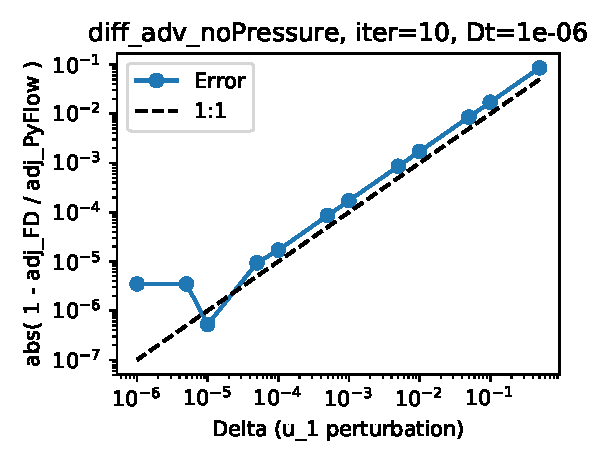
\includegraphics[width=0.475\textwidth]{Figures/errorCvg_diff_adv_noPressure_iter10_dt1e-06.pdf}}
  \subfloat[Viscous and convective terms, $n_\mathrm{iter}=10$, $\Delta t=10^{-5}$\,s]{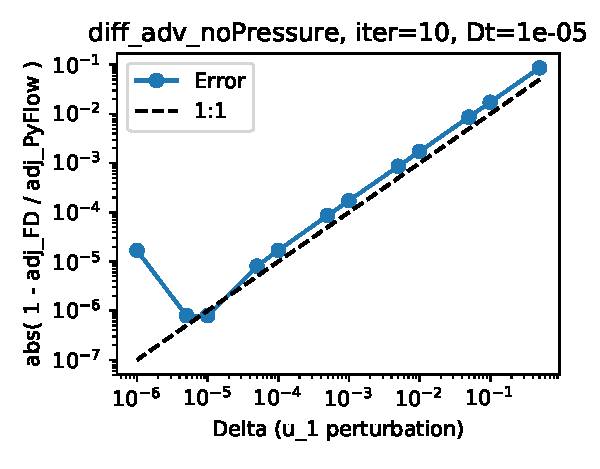
\includegraphics[width=0.475\textwidth]{Figures/errorCvg_diff_adv_noPressure_iter10_dt1e-05.pdf}}\\
  
  \subfloat[Navier-Stokes equations, $n_\mathrm{iter}=10$, $\Delta t=10^{-6}$\,s]{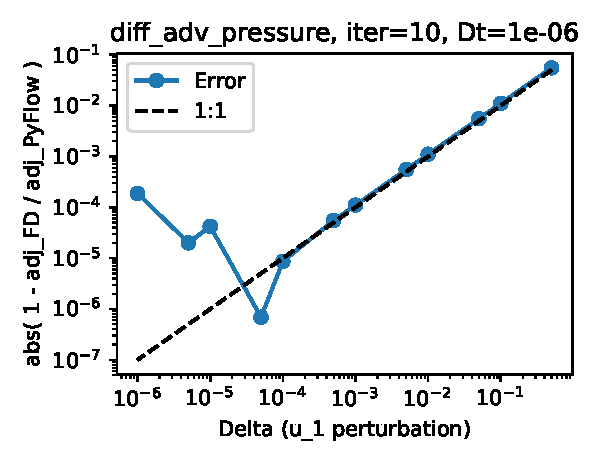
\includegraphics[width=0.475\textwidth]{Figures/errorCvg_diff_adv_pressure_iter10_dt1e-06.pdf}}
  \subfloat[Navier-Stokes equations, $n_\mathrm{iter}=10$, $\Delta t=10^{-5}$\,s]{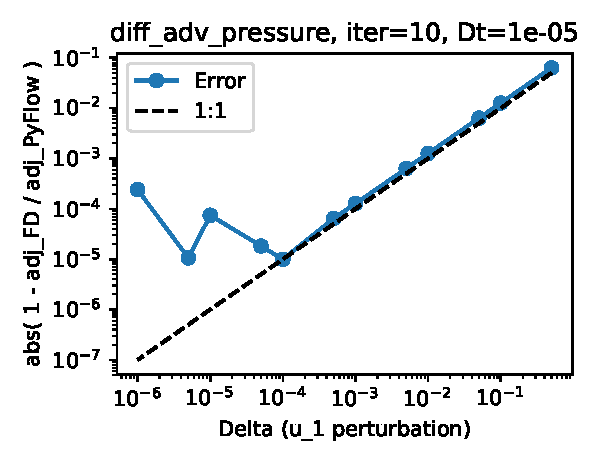
\includegraphics[width=0.475\textwidth]{Figures/errorCvg_diff_adv_pressure_iter10_dt1e-05.pdf}}

  \caption{Convergence of the adjoint solution. The pressure solver is omitted in the top row and included in the bottom row. The total solution time ($n_\mathrm{iter}\cdot\Delta t$) is increased by a factor of 10 in the right column.}
\end{figure}


\end{document}
